\section{Objectives, scenarios and baseline architecture}\label{sec:objectives}

\subsection{Objectives of Activity 4}
Activity~4 develops motion planners for teams of mobile manipulators and industrial arms working in dynamic, human-shared environments, integrated in the COMAU MI.RA/Dexter platform and in the Core IPC. The project targets are autonomous plan generation in all working conditions (joint and Cartesian), a reduction of about 30\% of the execution time of interaction tasks with respect to state-of-the-art planners, and safe adaptation of the velocity to the working conditions (Project Description, \S A.4.4).

\subsection{Baseline architecture}
The new generation of controllers relies on two computing units (Figure~\ref{fig:ipc}). The \emph{Open IPC} hosts the programming tools (MI.RA/Dexter, ROS\,2), the sensing and the motion planner, and acts as the bridge between the non-real-time and the real-time worlds. The \emph{Core IPC} runs the hard real-time motion control, the micro-interpolation (high-rate real-time motion planner) and all safety rules. The original plan combined informed sampling-based planning in the Open IPC with an MPC micro-interpolator in the Core IPC.

\begin{figure}[h]
\centering
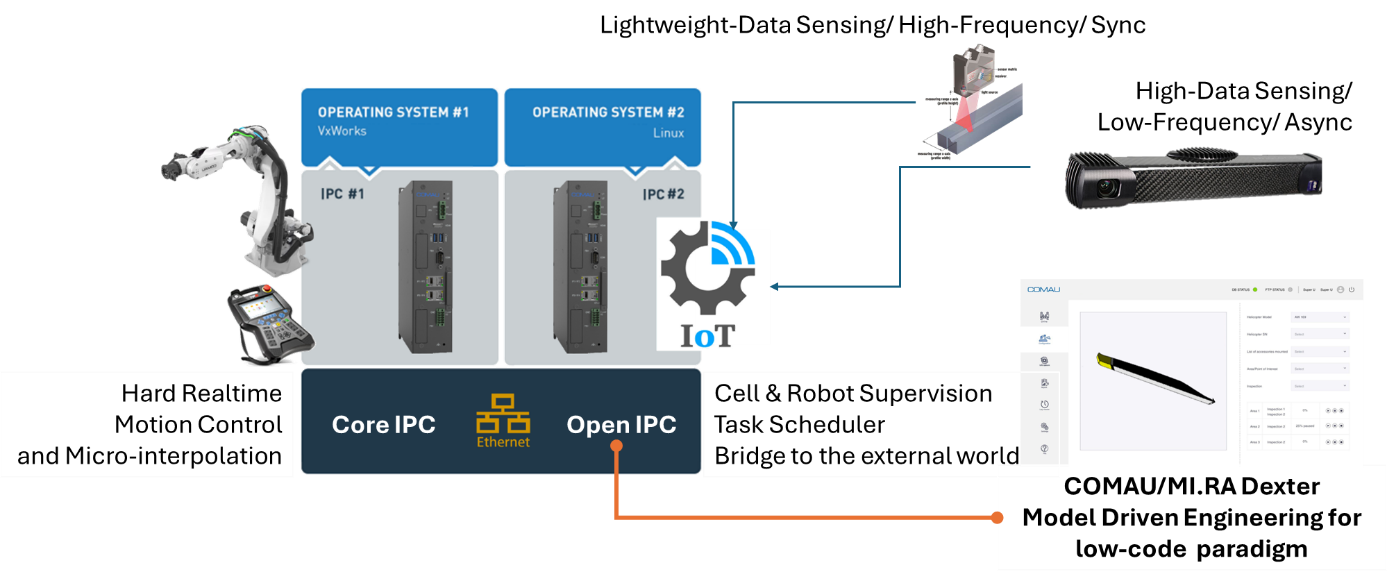
\includegraphics[width=0.9\linewidth]{figures/ipc_architecture.png}
\caption{Baseline architecture of the new generation of robot controllers (from the Project Description): the Open IPC provides programming tools, motion planner and the bridge to cell and sensing; the Core IPC oversees control loops, micro-interpolation and safety rules.}\label{fig:ipc}
\end{figure}

\subsection{Reference application}
Arc welding of very large metal structures by an industrial arm mounted on an AGV (optionally on an interpolated linear axis). The AGV is placed at a station and the arm welds a portion of the structure; base motion interpolated with the arm during welding is a secondary, theoretically relevant option. The task is \emph{under-constrained}: the seam point must be reached exactly, the torch axis may lie within a cone of about $10^\circ$ around the nominal direction (possibly anisotropic between work and travel angle), the rotation about the torch axis is almost always free, and the travel speed must stay constant within $\pm10\%$ along the whole seam. Because of the size of the structure the arm may have to change configuration: stop, retract, reconfigure, approach and restart about 1\,cm before the detach point. Seam segmentation and a raw positioning of the manipulator that reduces reconfiguration risk are standard industrial practice and are made explicit in the updated pipeline.

\subsection{Requirements}\label{sec:req}
\begin{enumerate}[label=R\arabic*.]
\item \textbf{Exact task, free redundancy.} Task constraints (position, axis) are hard; tolerances (cone, roll, external axes, base) are exploited as optimisation freedom~\cite{demaeyer2017descartes,chen2025cooptimization}.
\item \textbf{Speed band.} Travel speed within a fixed band ($\pm10\%$) under joint velocity, acceleration and jerk limits~\cite{lange2016pathaccurate}.
\item \textbf{Planned reconfigurations.} Fewest stop--reconfigure--restart cycles, with planned transfer motions and restart overlap~\cite{yin2024dpbreakpoints,wang2025anytimetracking}.
\item \textbf{Optimal task localisation.} Station / base / rail placement chosen so that whole task segments are feasible~\cite{weingartshofer2021tcpbase,wachter2024tcpbase}.
\item \textbf{Registration.} Mobile platforms on large workpieces show centimetre-level errors without local registration~\cite{zhao2021mobilemachining}; plans are executed on the locally registered task (seam scan~\cite{wang2026torchposture}, Activity~3).
\item \textbf{Human-shared space.} ISO/TS 15066-aware costs and certified speed adaptation~\cite{faroni2022safetyaware,gursoy2026cosmik}.
\item \textbf{Robot-agnostic.} Any serial arm (non-cuspidal or cuspidal~\cite{elias2025cuspidal}), joints with range beyond $\pm\pi$, external linear/rotary axes, mobile bases.
\item \textbf{Industrial integration.} Deterministic, repeatable outputs; dockerised actions in MI.RA/Dexter; hard real-time Core IPC.
\end{enumerate}
